\documentclass[12pt,aspectratio=43]{beamer}

% 自訂字體的封包
\usepackage{fontspec}

% 導入圖形與表格的封包
\usepackage{graphicx}
\usepackage{booktabs}

% 導入多張圖片動畫撥放
\usepackage{animate}

% 排列多個子圖形的封包
\usepackage{subfigure} 

 % 提供進階數學環境與公式排版
\usepackage{mathtools, amsmath, amsfonts, amsthm, latexsym} 

%% 設定中文字體
\usepackage{xeCJK}
\setCJKmainfont[AutoFakeBold=3.5 , AutoFakeSlant=0.2]{標楷體}
\setmainfont{Times New Roman}
\XeTeXlinebreaklocale "zh"
\XeTeXlinebreakskip = 0pt plus 1pt

% 自訂字體顏色的封包
\usepackage{color} 

% 圖表自動編號的封包
\usepackage{caption} 

% 允許表格的一格能多列呈現的封包
\usepackage{multirow} 

% 可指定表格排版的封包
\usepackage{array}

% 翻轉表格的封包
\usepackage{lscape} 

% 序列標號
\usepackage{enumerate} 

%% 設定自動編號
\setbeamertemplate{caption}[numbered]

%% 自訂顏色
\definecolor{Myblue}{RGB}{57,108,144}
\definecolor{Default_Blue}{RGB}{52,51,171}

% (動畫)字會若隱若現的顯示
\beamersetuncovermixins{\opaqueness<1->{45}}{\opaqueness<1->{95}} 

% 設定中文的標籤
\renewcommand{\figurename}{圖}
\renewcommand{\tablename}{表}

% 排版形式 
\mode<presentation>{
\usetheme{Berlin}
% enumerate 及 item 的形狀
\setbeamertemplate{itemize items}[triangle]
% 調整外框形式的字體大小
\setbeamerfont{headline}{size=\scriptsize}
\setbeamerfont{footline}{size=\scriptsize}
% 取消右下方的跳轉工具列
\setbeamertemplate{navigation symbols}{}
% 取消上方導覽列（headline）
\setbeamertemplate{headline}{}
% 自定義2：清除外框下緣但僅出頁碼
\setbeamertemplate{footline}[page number] 
% 顏色主題
\usecolortheme{dove}
% 設定頁面邊界
\setbeamersize{text margin left=0.2cm, text margin right=0.2cm}
\special{papersize=\the\paperwidth,\the\paperheight}
\providecommand{\tabularnewline}{\\}
}

\title{\fontsize{24pt}{20pt}統計專論（三）0224 HW}
\author{\fontsize{12pt}{0pt}黃丞暘}
\institute{\fontsize{12pt}{0pt}國立東華大學應用數學統計所}
\date{March 3, 2026}

\begin{document}

% 封面
\begin{frame}
  \titlepage
\end{frame}

% 目錄
\begin{frame}{\textbf{目錄}}
  \tableofcontents
\end{frame}


% 韋伯分配
\section{Weibull Distribution}
\subsection{PDF \& Parameters}
\begin{frame}[t]{\textbf{Weibull Distribution} -- PDF \& Parameters}
\linespread{1.5}

{\Large 常用來描述產品的壽命／故障時間}
  \begin{itemize}
    \item pdf: $ f(x;a,b)=\frac{b}{a}\left(\frac{x}{a}\right)^{b-1}\exp\!\left[-\left(\frac{x}{a}\right)^b\right],\quad x\ge 0,\quad a,b>0 $
    \begin{enumerate}[]
        \item $a$ 決定尺度（scale），$b$ 決定形狀（shape）
        \item Note: 當 $b=1 \Rightarrow f(x)=\frac{1}{a}e^{-x/a}$ , 即指數分配
    \end{enumerate}
  \end{itemize}

  \begin{columns}[c,onlytextwidth]
    \begin{column}{0.35\textwidth}
      \vfill
      cdf: $ F(x)=1-\exp\!\left[-\left(\frac{x}{a}\right)^b\right] $
      存活: $ S(x)=\exp\!\left[-\left(\frac{x}{a}\right)^b\right] $
    \end{column}

    \begin{column}{0.65\textwidth}
      \centering
      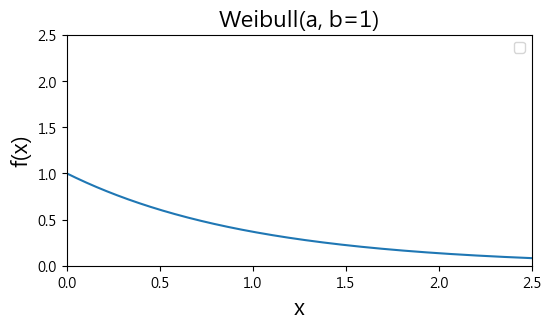
\includegraphics[width=0.7\linewidth]{Exponentialpdf.png}\\
      愈高表示愈多樣本會在該時間x附近失效；\\往右愈低表示愈晚失效的樣本愈少
    \end{column}
  \end{columns}
    \vspace{-0.2cm}
    % \item cdf: $ F(x)=1-\exp\!\left[-\left(\frac{x}{a}\right)^b\right] $
\end{frame}

\subsection{Reliability \& Hazard}
\begin{frame}[t]{\textbf{Weibull Distribution} -- Reliability \& Hazard}
  \begin{itemize}
        \item $b<1$：$f(x)$ 在靠近 $0$ 的位置較尖、右尾較長
        \item $b=1$：$f(x)=\frac1a e^{-x/a}$
        \item $b>1$：$f(x)$ 在 $0$ 附近趨近 0，出現峰值後再下降
  \end{itemize}
\begin{figure}
    % 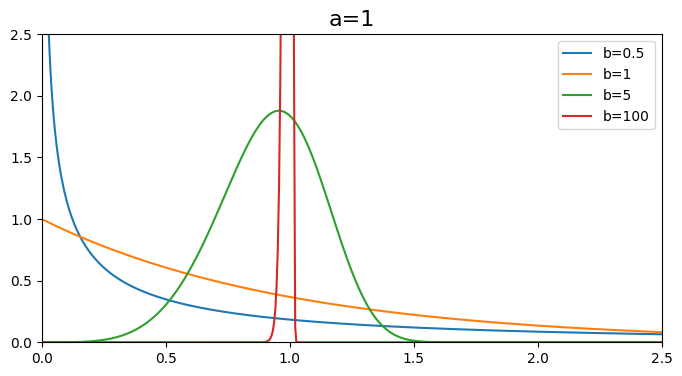
\includegraphics[scale=0.4]{Weibullpdf.png}
    \animategraphics[controls,loop,width=0.7\linewidth]{12}{weibull_anim/frames/frame_}{001}{060}
\end{figure}
\end{frame}


% 卜瓦松分配
\section{Poisson Distribution}
\subsection{PMF \& Properties}
\begin{frame}[t]{\textbf{Poisson Distribution} -- PMF \& Properties}
\linespread{1.5}

{\large 常用來描述固定時間／固定區域內事件發生的次數}
  \begin{itemize}
    \item pmf: $ P(X=x;\lambda)=\frac{\lambda^{x}e^{-\lambda}}{x!},\quad x=0,1,2,\ldots,\ \lambda>0 $
    \begin{enumerate}[]
      \item $\lambda$ 為平均發生次數，同時也是期望值
      \item 事件之間彼此獨立，且短時間內同時發生很多次的機率很小
      \item x 愈大表示同一段時間內發生的次數愈多；$\lambda$ 愈大整體分佈右移且更分散
    \end{enumerate}
    \item Properties
    \begin{enumerate}[]
      \item mean(期望值)：$ \mathbb{E}[X]=\lambda $
      \item variance(變異數)：$ \mathrm{Var}(X)=\lambda $
      \item $ X_1+X_2 \sim \mathrm{Poi}(\lambda_1+\lambda_2) $
    \end{enumerate}
  \end{itemize}

\end{frame}

\subsection{PMF \& Lambda}
\begin{frame}[t]{\textbf{Poisson Distribution} -- PMF \& Lambda}
  \begin{itemize}
    \item $\lambda$ 小：大多集中在 $k=0,1,2$（事件不常發生）
    \item $\lambda$ 中等：常見次數接近平均
    \item $\lambda$ 大：分佈右移且更寬（平均次數更高且波動更大）
  \end{itemize}
  \begin{figure}
      \animategraphics[controls,loop,width=0.6\linewidth]{12}{poisson_anim/frames/frame_}{001}{060}
  \end{figure}
\end{frame}

% END
\begin{frame}[plain] % 產生無外框的頁面
	\begin{center}
		{\Huge The End}
		\bigskip\bigskip 
		
		{\LARGE Questions}
	\end{center}
\end{frame}
\end{document}
